\documentclass{article}
\usepackage[utf8]{inputenc}
\usepackage[top=2.5cm, bottom=2.5cm, left=2cm, right=2cm]{geometry}
\usepackage{amsmath}
\usepackage[toc,page]{appendix}
\usepackage{minted}
\usepackage{url}
\usepackage{hyperref}
\usepackage{graphicx, caption, subfigure, wrapfig}
\hypersetup{colorlinks,citecolor=black,filecolor=black,linkcolor=black,urlcolor=black}
\setlength\parindent{0pt}
\newcommand{\vect}[1]{\boldsymbol{#1}}

\graphicspath{{Pictures/}} % Specifies the directory where pictures are stored

\begin{document}
\title{Multiscalorithms\\
		\small Integrating Multiscale Dynamical Systems\\~\\
        \small Numerical Algorithms - Final Assignment}
\author{Martijn van Beest, Jaro Camphuijsen, Rahiel Kasim\\
~~~~~(11059184) \hfill ~~~(6042473) \hfill (1044539)~~~}
\maketitle

\tableofcontents
\section{Introduction}
The model by Ford, Kac and Zwanzig \cite{fordkac} describes a dynamical system with a multiscale character. We have one distinguished particle that moves in a heatbath with many other $N$ particles. These $N$ particles don't interact with each other, only with the distinguished particle. The particles in the heatbath behave as harmonic oscillators. Finally, the distinguished particle moves in the potential $V(q) = \frac{1}{4} (q^2 - 1)^2$. This potential is plotted in figure \ref{fig:pot}. A particle in the potential would be pushed to the middle, where the potential is lowest.
\begin{figure}
\center{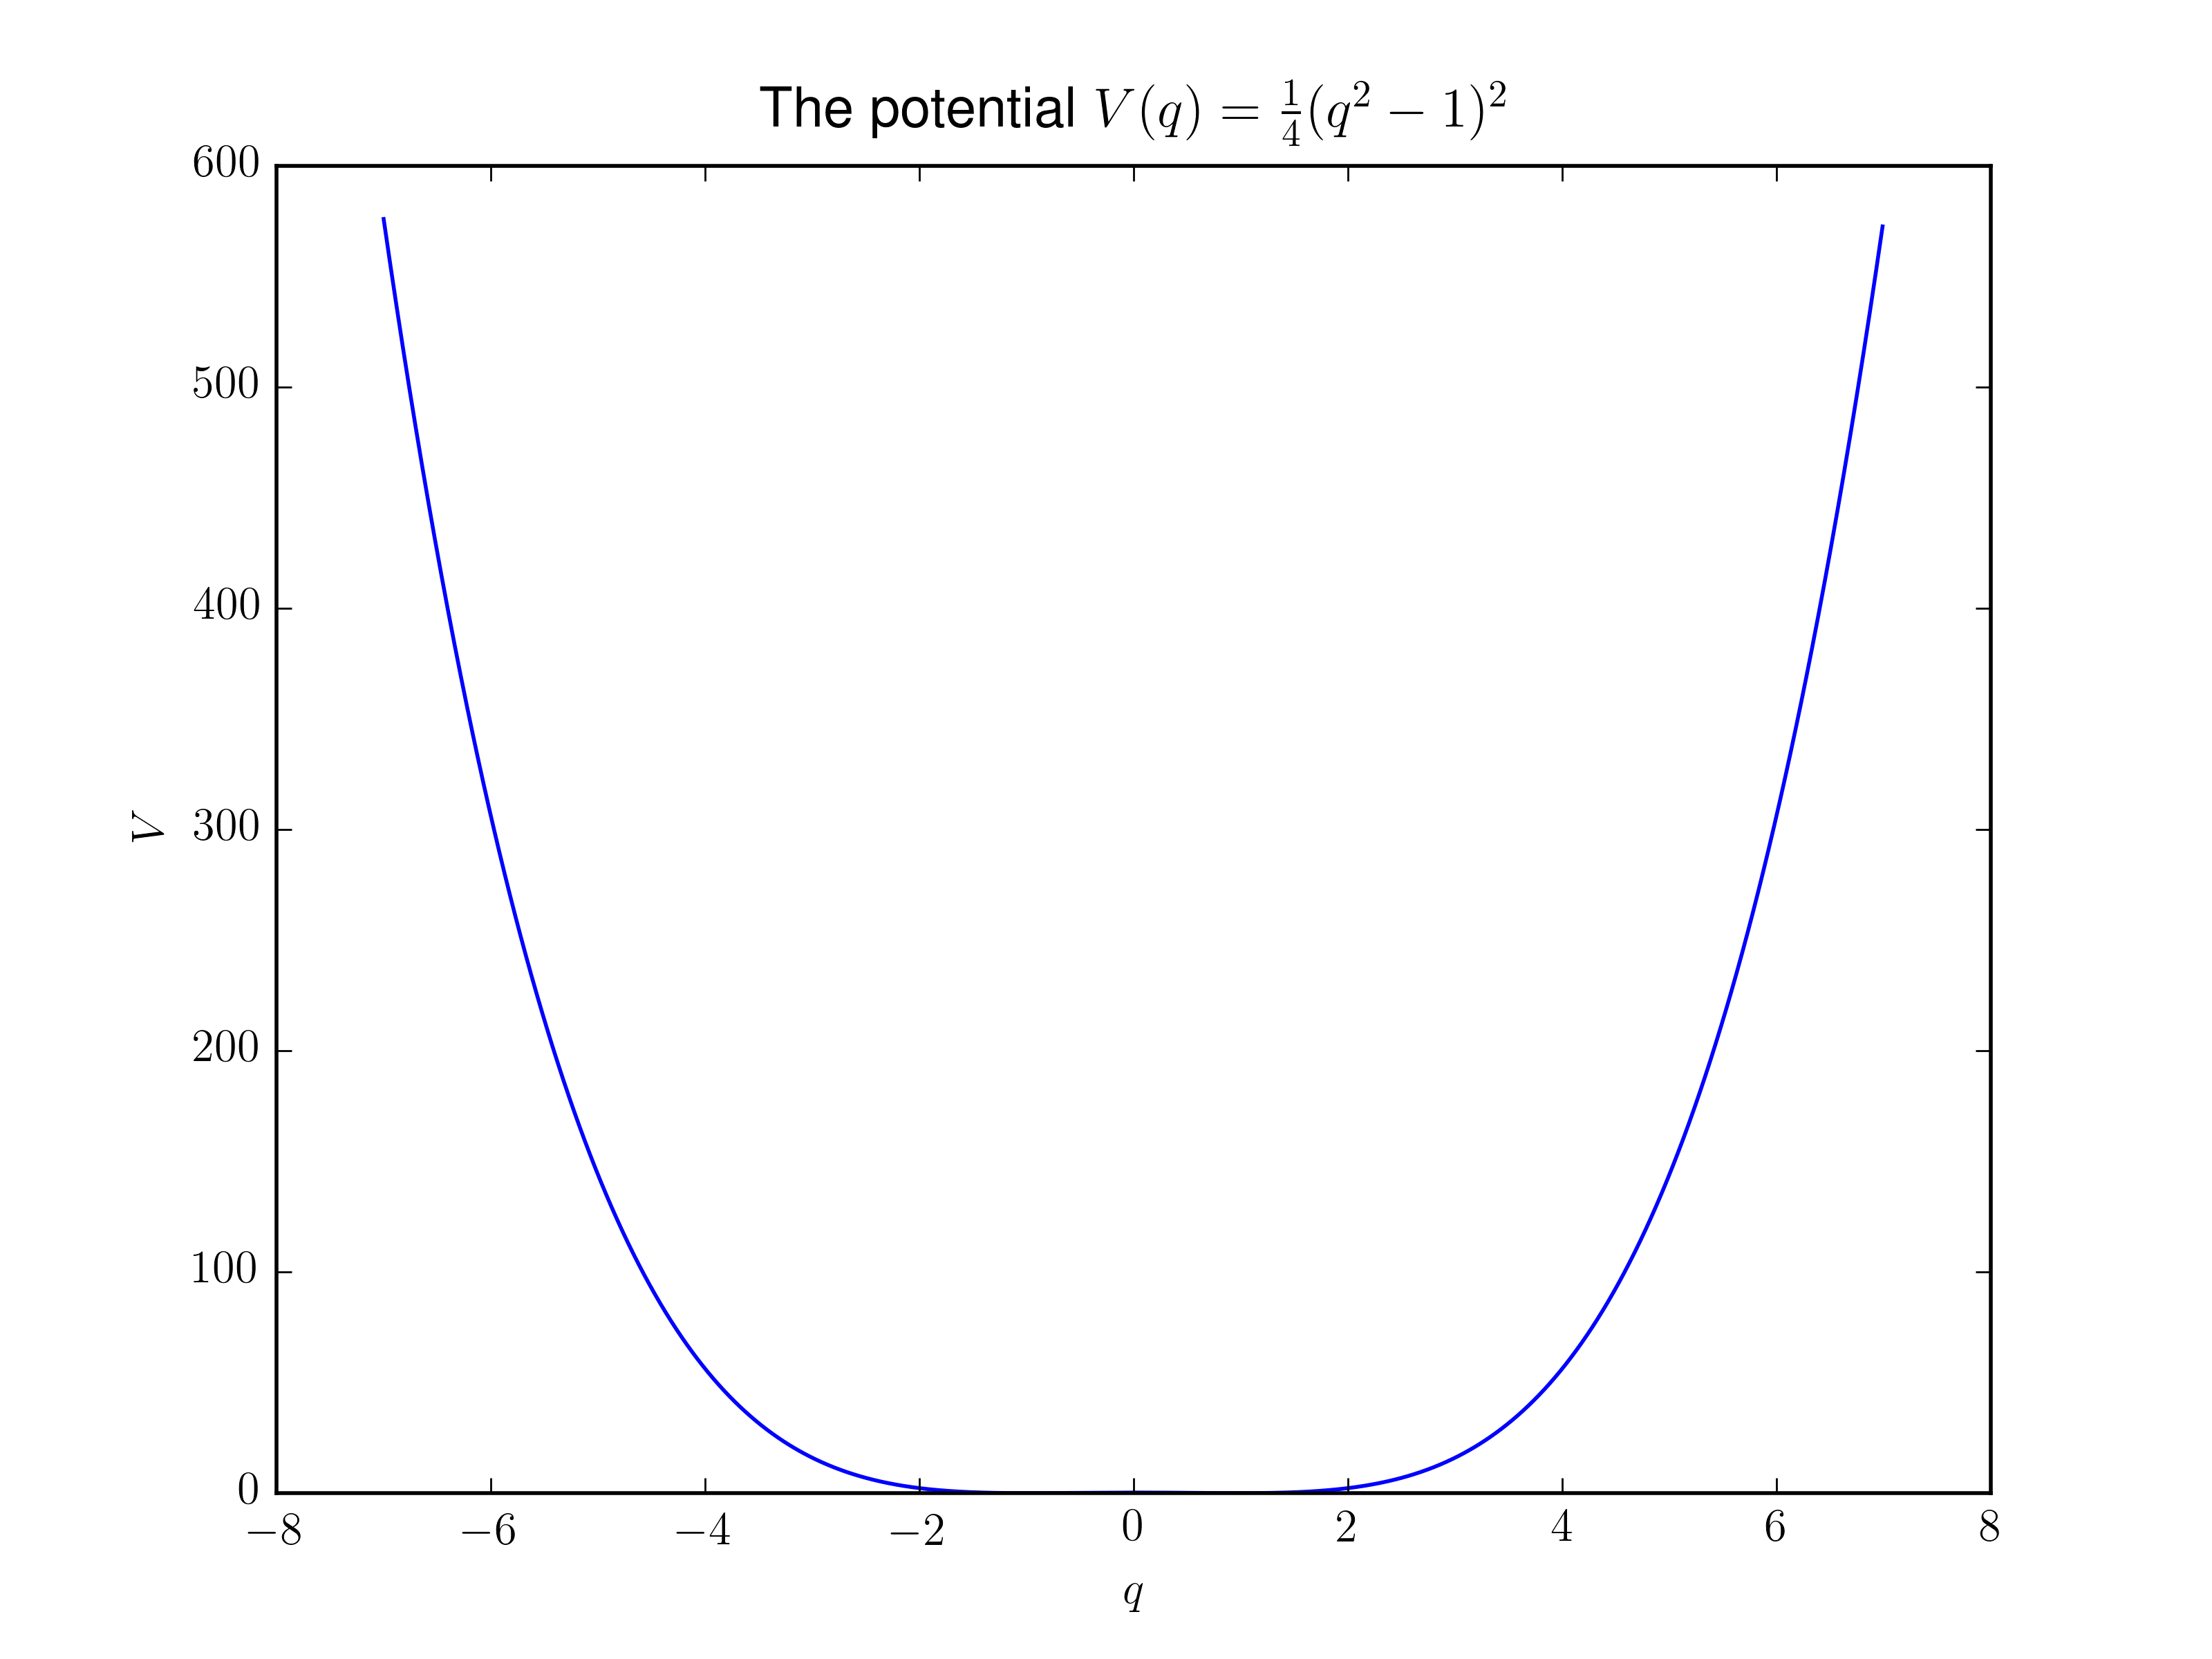
\includegraphics[height=7cm]{potential}}
\caption{The potential of the system.}
\label{fig:pot}
\end{figure}

\section{Problem Description}
The problem at hand is that of solving the following system of ordinary differential equations (ODE):
\begin{align}
\begin{split}
\dot q &= p\\
\dot p &= - V\prime(q) + \gamma ^2 \sum \limits_{j=1}\left( u_{j} -q\right)\\
\dot u_j &= v_j\\
\dot v_j &= -j^2(u_j - q)
\end{split}
\label{eq:ODE}
\end{align}

This system represents a particle in a heat bath, where $q$ and $p$ are respectively the position and momentum of the single distinguished particle and $u_j$ and $v_j$ are respectively the positions and momenta of each of the $N$ harmonic oscillators in the heat bath. \\ 
It was shown by Kac and Ford \cite{fordkac} that the distinguished particle in this model exhibits motion similar to Brownian motion under influence of the heat bath's interactions in the limit of $N \rightarrow \infty$. However since $\dot v_j$ depends on the index $j$ of harmonic oscillators, the model becomes very stiff for large $N$.  

\section{Methods}\label{sec:methods}
When solving ODE's we use so called numerical integrators to solve an initial value problem (IVP). We calculate the values of the function at the $n$th time step from the values at previous step(s). This gives us an approximation of a single unique solution to the ODE depending on the initial conditions.  Although we do not necessarily find a true solution to the ODE, we track the solution by extrapolating the current solution track at each point to the next time step by integration. In the limit of step size $h\rightarrow \infty$ (also implying infinite computation time), this gives the unique solution to the initial value problem.\\ 

We've looked at and analyzed several numerical integrators, as we shall see now.

\subsection{Forward Euler}
\label{ssec:feuler}
Starting at the simplest of integration schemes, the implementation of the Forward Euler scheme can be found in Appendix \ref{app:calc}. We can replace the value of some function $y(t)$ at $(t+h)$ by the Taylor series:
\begin{equation}
\mathbf{y}(t+h) = \mathbf{y}(t) + h \mathbf{y}'(t) + \frac{1}{2} h^2 \mathbf{y}''(t) + \dots
\end{equation}
The Forward Euler method is a first order explicit integration scheme, where first order means that we drop second and higher order terms in the Taylor series approximation (first order also means that the local error at every step is of size $O(h^2)$), so we end up with:
\begin{equation}
\mathbf{y}(t+h) = \mathbf{y}(t) + h \mathbf{y}'(t),
\end{equation}
Here $\mathbf{y}'(t)$ is simply the system of expressions for the first derivatives from the differential equation as shown in \eqref{eq:ODE} evaluated at the current time step, while $\mathbf{y}(t)$ are simply the values at the current time step. Adding the size of the time step times the derivative is the simplest form of integration. \\
The forward Euler method has a very limited stability, especially for stiff equations like this problem. This means that even while the exact solution converges quickly to a steady state solution, integration with forward Euler results in very rapid divergence.  

\subsection{Backward Euler}
The forward Euler method only uses information from the current time step to calculate the next step. This makes the method very unstable. We can also derive the implicit backward Euler method in the same way as the forward version. By taking the first two terms of the backward Taylor series at time $(t-h)$:

\begin{align}
\begin{split}
\mathbf{y}(t-h) &= \mathbf{y}(t) - h \mathbf{y}'(t)\\
\mathbf{y}(t) &= \mathbf{y}(t - h) + h \mathbf{y}'(t)\\
\mathbf{y}(t + h) &= \mathbf{y}(t) + h \mathbf{y}'(t + h)
\end{split}
\label{eq:beuler}
\end{align}

However this requires to evaluate the system at a time of which there are no function values yet. We can solve the resulting set of non-linear equations using Newton's method, of which the implementation can also be found in appendix \ref{app:calc}. \\ 
Newton's method is used to solve the system of backward Euler equations:

\begin{align}
\mathbf{g}(\mathbf{y}(t+h))  
 &= \mathbf{y}(t + h) - \mathbf{y}(t) - h \mathbf{f}(\mathbf{y}(t + h)) = 0
\end{align}

where $\mathbf{y}'(t+h)$ in \eqref{eq:beuler} is replaced by $\mathbf{f}(\mathbf{y}(t + h))$ with $\mathbf{f(y)}$ the differential equations evaluated with the values $\mathbf{y}$. Since $\mathbf{y}(t)$ is known, the only variable vector in the equation is $\mathbf{y}(t+h)$ and thus we can solve this system $\mathbf{g}$ of non-linear equations with Newton's method. The system of non-linear equations is replaced with the truncated Taylor series of the system which is a system of linear equations:
\begin{align}
\mathbf{g}(\mathbf{y} + \mathbf{s}) \approx \mathbf{g}(\mathbf{y}) + \mathbf{J}_g (\mathbf{y})\mathbf{s}
\end{align}

Here $\mathbf{J}_g$ is the Jacobian matrix of the system $g$. The solution to this linear system is taken as an approximation to the solution of the non-linear system, so it has to be solved iteratively to converge towards the true solution up until some specified tolerance.
Newton's method needs an initial guess, for which we can use either the previous step in the integration process or the next step calculated using an explicit integration method.
Calculating the Jacobian of the system is computationally intensive, as it consists of $(2N + 2)^2$ components, and it has to be performed many times per time step. 
This makes backward Euler only feasible when it is possible to make $h$ very big. This is the case for the current problem of which the stiffness increases with the number of harmonic oscillators $N$. 
Backward Euler has the inverse stability region of forward Euler and is therefore especially suited for stiff equations as it is unconditionally stable. It will reach the stable solution for arbitrary step size $h$.  \\
While unconditionally stable, backward Euler is still of first order and will therefore have a local error comparable to forward Euler. In this sense it is not necessary to set a tolerance on Newton's method lower than order $\mathcal{O}(h^2)$, since the error in the integration will always be $\mathcal{O}(h^2)$. To improve this local error we need to increase the order of the integration scheme.

\subsection{Runge-Kutta 4}
Integration schemes from the explicit Runge-Kutte family are of the form
\begin{align}
\begin{split}
\mathbf{y}_{k+1} &= \mathbf{y}_k + \sum\limits_{i=1}^s b_i \mathbf{k}_i
\label{eq:rkfam}
\end{split}
\end{align}
where $\mathbf{k}_i$ are the intermediate evaluations of the system of derivatives at the values of the current time step adjusted by the previous intermediate result. The two best known explicit Runge-Kutta methods are the forward Euler method, which is of order 1 and explained in section \ref{ssec:feuler}, and Runge-Kutta of fourth order (RK4) which is given below: 

\begin{align}
\mathbf{y}_{k+1}& = \mathbf{y}_k + \frac{h}{6}(\mathbf{k}_1 + 2\mathbf{k}_2 + 2\mathbf{k}_3 + \mathbf{k}_4)\\
~ \nonumber \\
\begin{split}
\mathbf{k}_1& = \mathbf{f}(t_k, \mathbf{y}_k)\\
\mathbf{k}_2& = \mathbf{f}(t_k + h/2, \mathbf{y}_k + (h/2)\mathbf{k}_1) \\
\mathbf{k}_3& = \mathbf{f}(t_k + h/2, \mathbf{y}_k + (h/2)\mathbf{k}_2) \\
\mathbf{k}_4& = \mathbf{f}(t_k + h, \mathbf{y}_k + h\mathbf{k}_3)
\end{split}
\end{align}

The implementation of this method is straightforward and the local error is $\mathcal{O}(h^5)$. This is a major improvement on forward Euler, however since it is still an explicit integration scheme, it is not unconditionally stable and will in the end diverge.
The implementation of RK4 can be found in appendix \ref{app:calc}. 

\section{Implementation}
The methods described in section \ref{sec:methods} are implemented using Python 3. The source code can be found in Appendices \ref{app:main} to \ref{app:sym}. The code is separated in three files. The file \texttt{main.py} contains the general setup and system initialization. The file \texttt{calc.py} contains the different integrator functions and finally the file \texttt{sym.py} contains symbolic functions to generate the Jacobian for the Backward Euler function.\\

All numerical integration is done vectorised, i.e. all vector operations are done at the same time. This implies that given big vectors or matrices, the matrix operations are done transparently over multiple CPU cores. The vector with the values of all variables ($\vect{y}$) is of the form 
\begin{align*}
\begin{pmatrix}
q \\ p \\ u_1 \\ \vdots \\ u_N \\ v_1 \\ \vdots \\ v_N
\end{pmatrix}
\end{align*}.
For large $N$ the size of $\vect{y}$ and even more so of the Jacobian $J$ become large. If we make new arrays of these sizes every time when we evaluate the system and Jacobian, then we spend a lot of time allocating these matrices in memory every time step. So as an optimization, we allocate the memory for the matrices once during initialization and then reuse it during the integration.

Forward Euler and the RK4 functions are pretty straightforward implementations of the schemes as described in section \ref{sec:methods}.\\

 The implementation of the backward Euler is a bit more extensive since we also need to implement Newton's method to solve the nonlinear system at each time step as well as the Jacobian matrix. As stated before, the Jacobian matrix is computationally expensive. We therefore compute the Jacobian matrix once beforehand in \texttt{sym.py}, and evaluate only the values that change for each time step. If we don't use this optimization, the computation time will exists for a major part of Jacobian computations. We use the \texttt{sympy} package to compute the Jacobian symbolically.
 
Another optimisation for the backward Euler scheme is in the choice of initial guess. Every time step we first do a step of Forward Euler and use its result as initial guess for Newton's method.

The implementation is also available online on GitHub \cite{github}.

\section{Results}
We've used $\gamma=1$ and $N=100$. The distinguished particle starts at $q=0$ with $p=0.1$ and the $N$ particles have $v_j(0)=0$ and $u_j(0) = 100 r_j$ for all $j$, where $r_j$ are randomly sampled from a normal distribution with mean 0 and variance 1.

We integrated the model with the three different integration methods. To see how they perform, we look at the value of $q$ integrated from $t=0$ to $t=10$ with a step size of $h=0.01$ and a tolerance for Newton's method of tolerance=$h^2 = 0.001$. The error from the Forward Euler method diverges, so we set those values to zero after its absolute value exceeds 20. The result can be seen in figure \ref{fig:compare}. We see that the Forward Euler method quickly diverges, it's value is cut off and set to zero so the other graphs stay visible in the same figure. The values for Runge-Kutta 4 and the backward Euler are mostly the same throughout the whole time period. From this we decided to continue comparing the explicit Runge-Kutta 4 with the implicit backward Euler. In this plot the integration time for RK4 was 0.59 CPU and wallclock seconds and backward Euler took 16.3 CPU and 4.1 wallclock seconds. Here we have not taken advantage of the fact that the Backward Euler scheme can handle bigger time steps than RK4.

\begin{figure}
\center{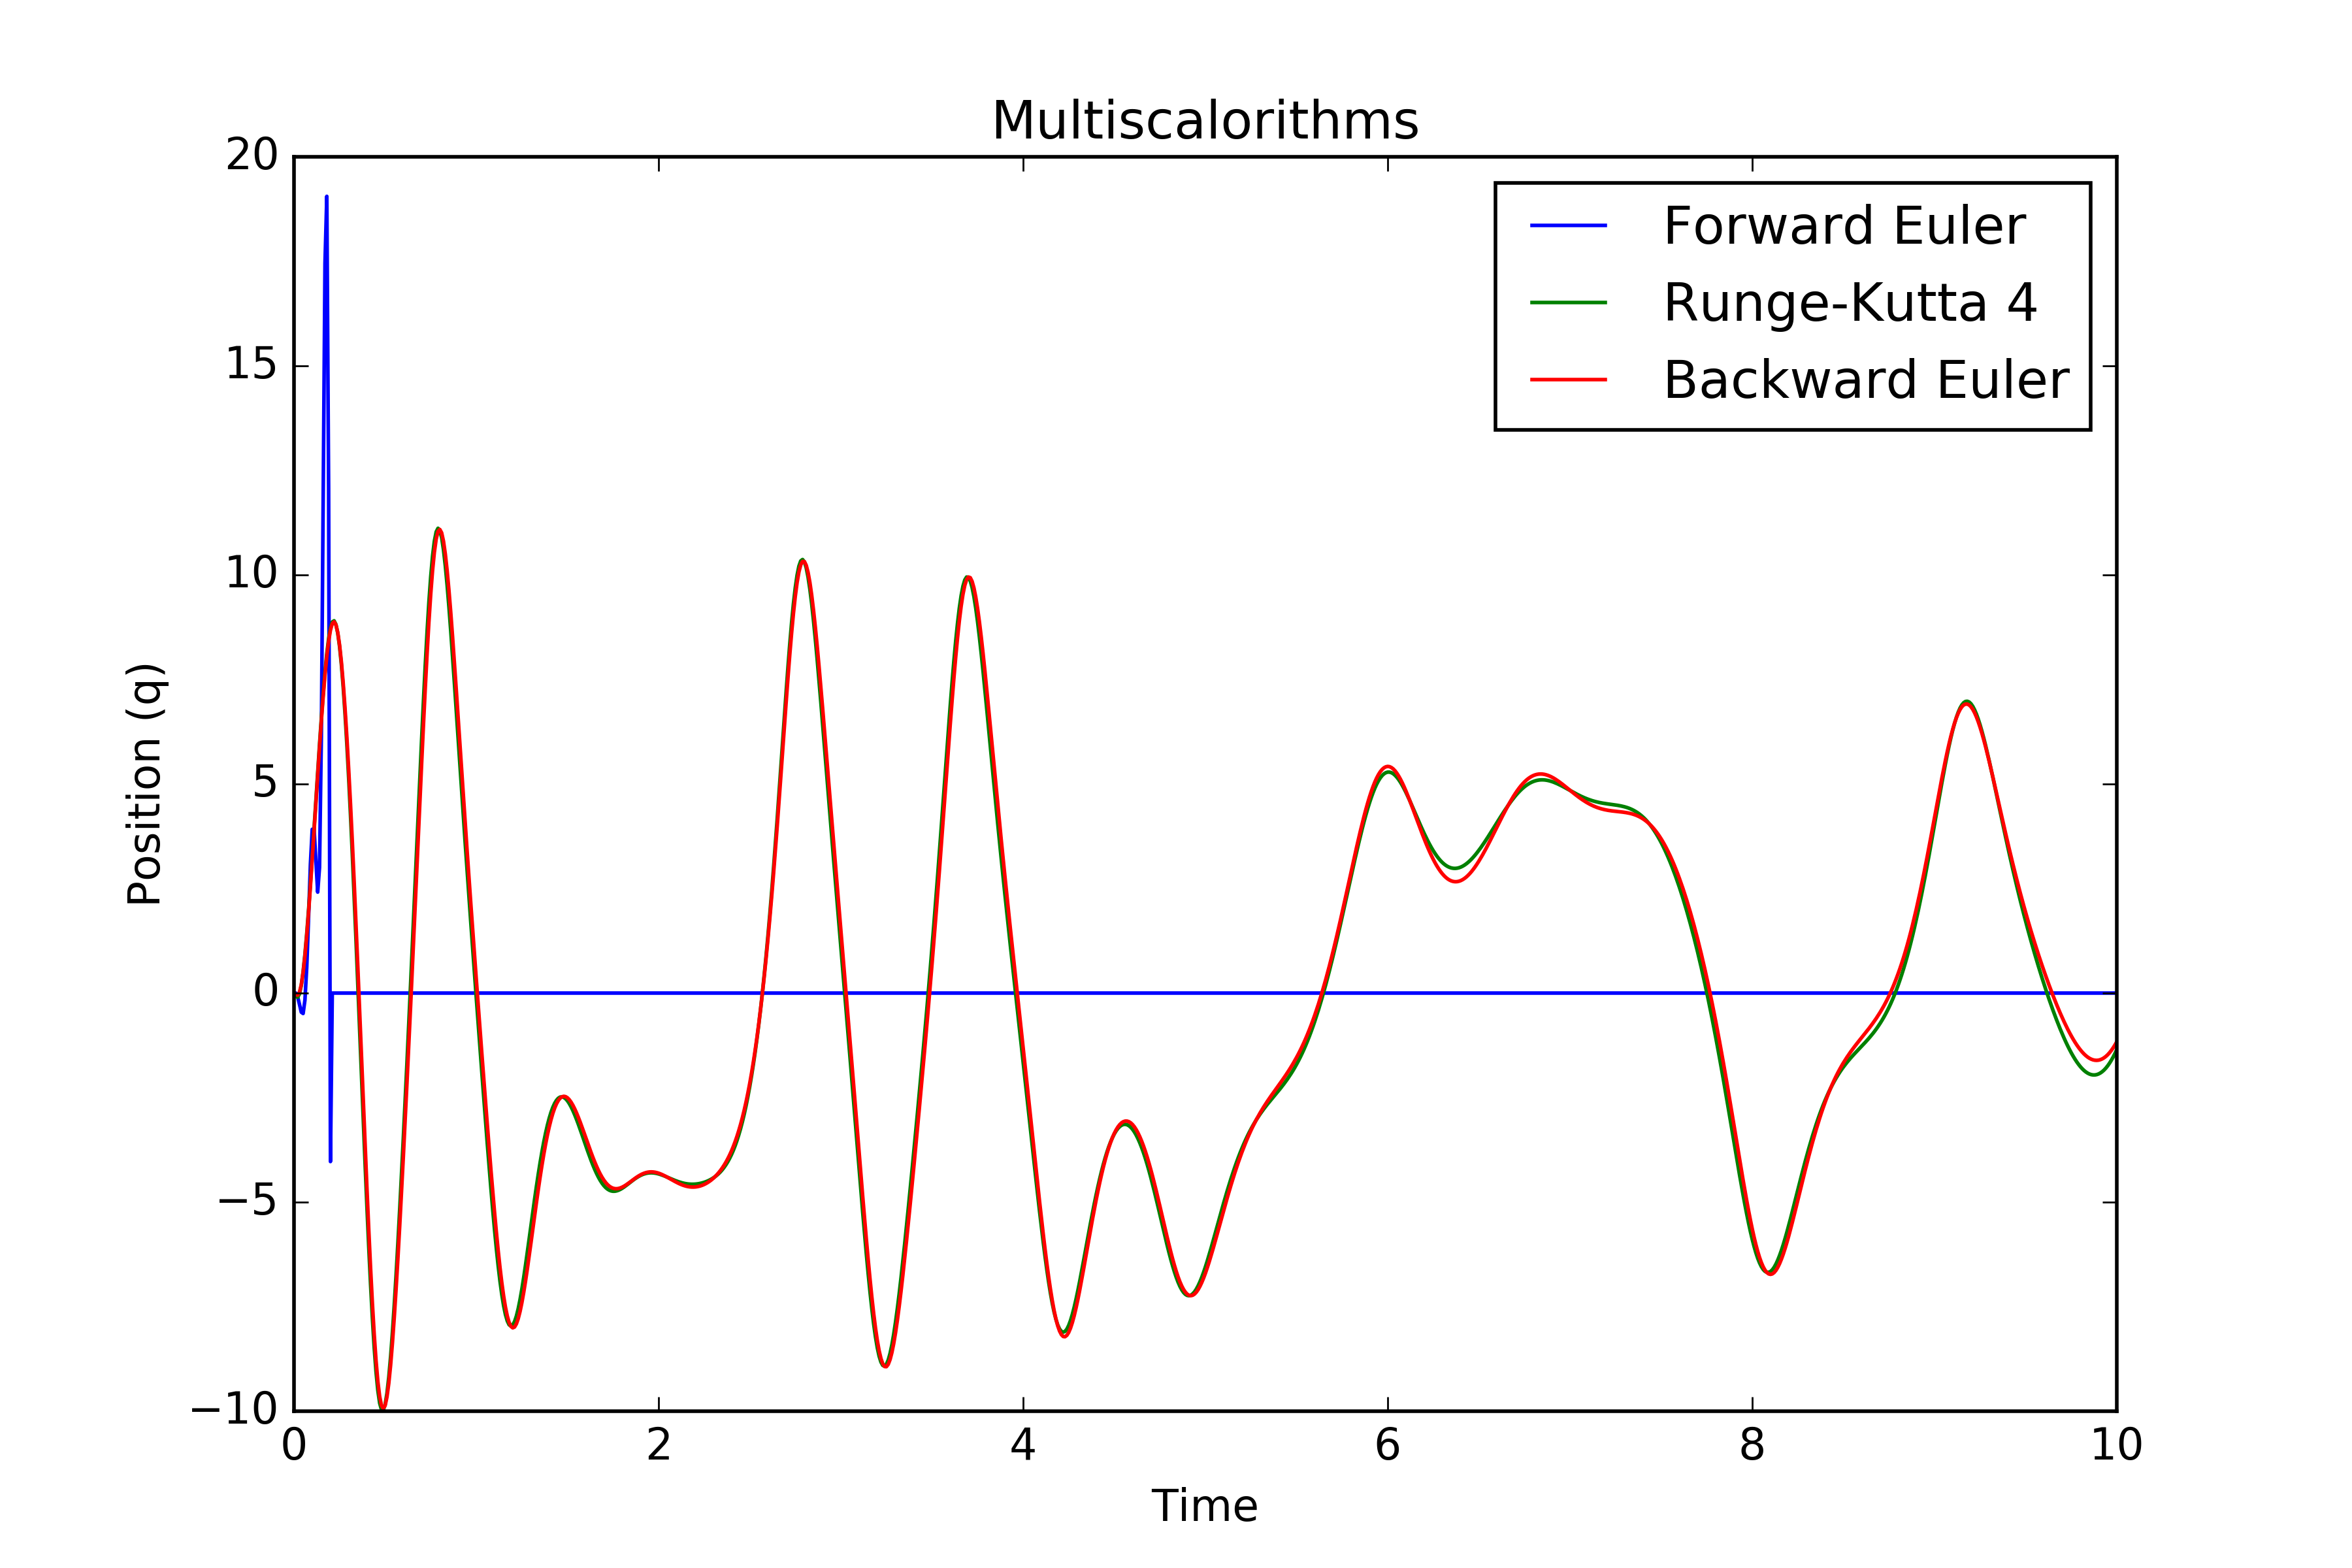
\includegraphics[height=8cm]{methods_position_comparison}}
\caption{The position of the distinguished particle over a small time period as calculated by the different integration schemes. The value of the Forward Euler is set to zero after its value exceeds 20 (because it diverges).}
\label{fig:compare}
\end{figure}

Taking another look at the potential in figure \ref{fig:pot} and the position of the distinguished particle in figure \ref{fig:compare}, we can interpret what happens. The distinguished particle is pushed out by the heatbath to the sides, but the potential pushes the distinguished particle back to the middle ($q=0$). This explains the oscillation in $q$.

To optimize the backward Euler method the initial guess of the Newton method can be chosen in an intelligent way. The simulation was run for increasing step size with constant number of steps for the last integration step as initial guess and with the next integration step using forward Euler as initial guess and CPU times were measured and shown in figure \ref{fig:newtInit}

\begin{figure}
\center{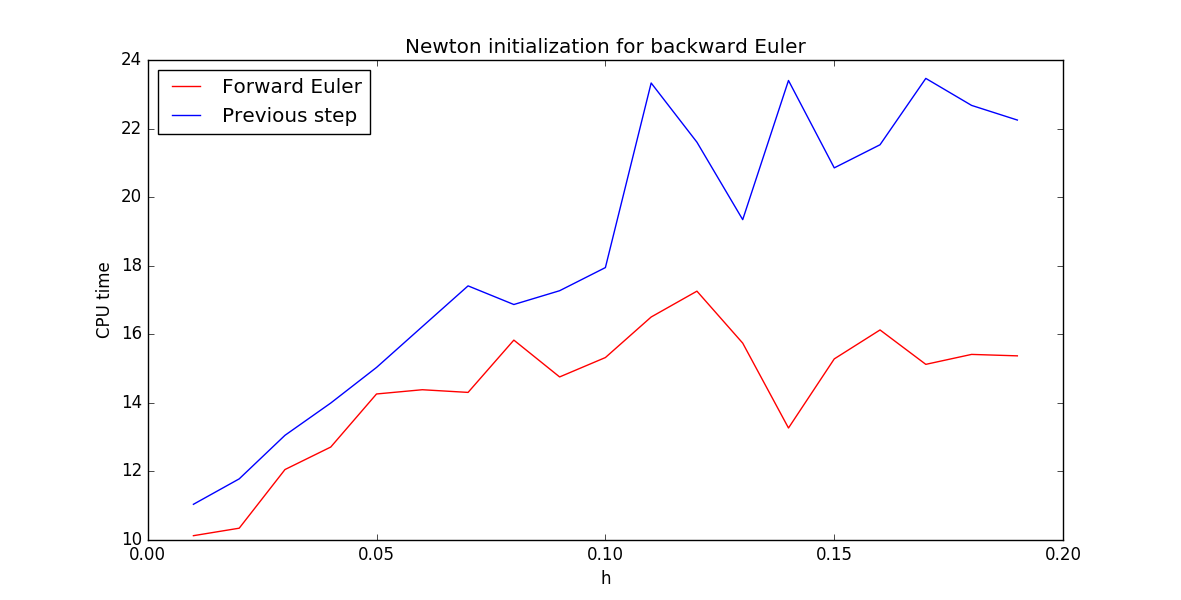
\includegraphics[height=8cm]{newtInit}}
\caption{Two methods were used for initializing the Newton method for solving the non-linear equations in backward Euler. Using the previous integration step as initial guess and using the explicit forward Euler method to compute the initial guess. Simulations were run for 1000 steps with increasing step size.}
\label{fig:newtInit}
\end{figure}

In measuring computational cost we make a distinction between CPU time and wallclock time. CPU time is the actual time a CPU has spent on the integration. This also means that two CPU's computing at the same time for 1 s would give a CPU time of 2 s. The other time we measure is the real time, or wall clock time.

Figure \ref{fig:compare-cpu-times} and \ref{fig:compare-wall-times} show comparisons in computation time between the RK4 method and backward Euler for $T=1000$ and $h=0.01$. Since the backward Euler method uses parallelization the cpu times in Figure \ref{fig:compare-cpu-times} are in fact the cpu times of 8 cores combined. If one is only interested in how much time a computation takes in total, figure \ref{fig:compare-wall-times} shows the elapsed wall time for both integration methods.

\begin{figure}[ht]
\center{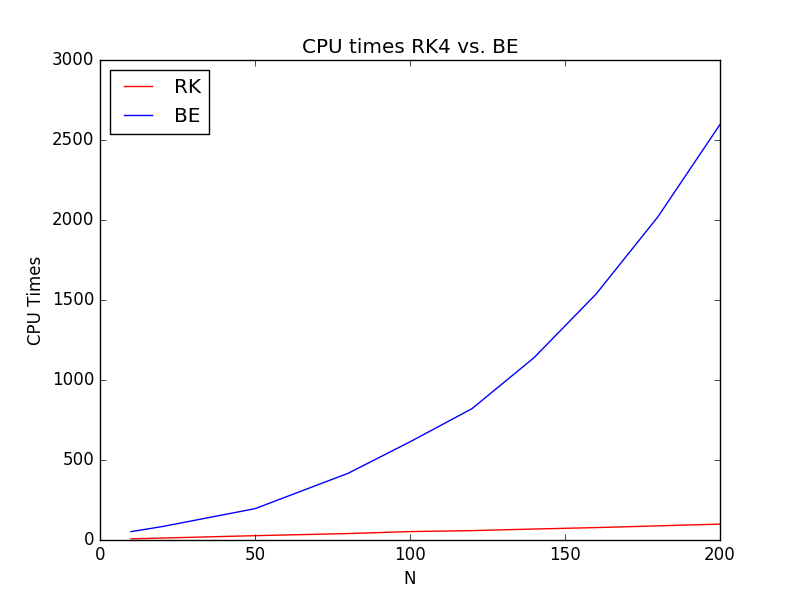
\includegraphics[width=0.8\textwidth]{compare-cpu-times}}
\caption{Comparison of CPU times (in seconds) between RK4 and BE for increasing values of $N$.}
\label{fig:compare-cpu-times}
\end{figure}

\begin{figure}[ht]
\center{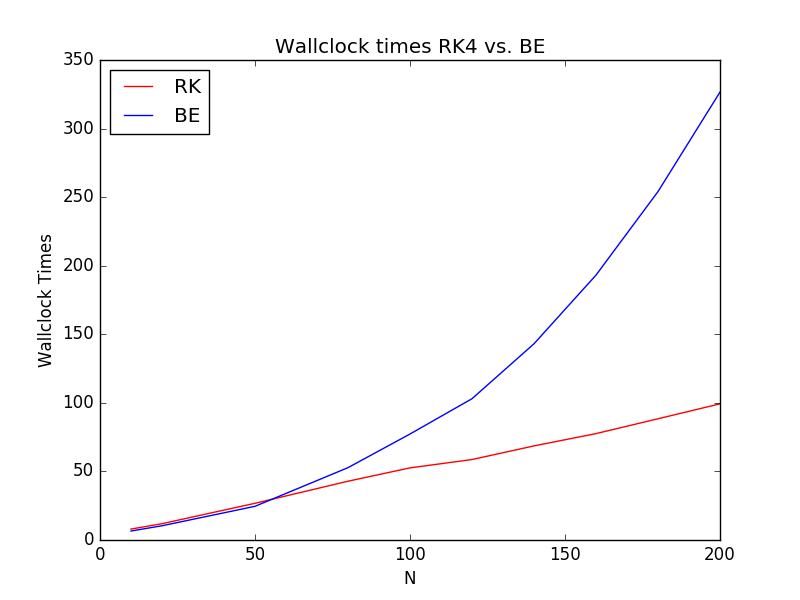
\includegraphics[width=0.8\textwidth]{compare-wall-times}}
\caption{Comparison of Wallclock times (in seconds) between RK4 and BE for increasing values of $N$.}
\label{fig:compare-wall-times}
\end{figure}


\section{Conclusion}
In figure \ref{fig:compare} it can be seen that the forward Euler method is least stable. After very short time the integration diverges and the integration is killed by our safety test. Both Runge-Kutta 4 and backward Euler remain stable for the full duration of the simulation, however we see a small difference which is probably due to backward Euler being of first order. However for this short simulation Euler took a CPU time of 16.3 while RK4 took 0.59. Also in figure \ref{fig:compare-cpu-times} and \ref{fig:compare-wall-times} the CPU and wallclock times are shown for increasing N. This shows the high computation costs for backward Euler due to the iterative solving of the system of equations as opposed to the simple value substitution in RK4. For small time steps and short simulation times RK4 outperforms all, but for backward Euler the step size can be set arbitrarily large while RK4 is bound to small step size to remain stable. And we could in principle choose our backward Euler step size for backward Euler such that its wall time is shorter than Runge-Kutta. \\

From figure \ref{fig:newtInit} we see that when using the combination of backward Euler with forward Euler as initial guess for the Newton method, for large step sizes the CPU time per step stabilizes, while with the naive initial guess of taking the previous integration step, the computation time keeps growing. As we increase the step size, the error induced by taking the initial guess of the previous integration step keeps growing while the more intelligent guess of the next forward Euler step is much closer to the solution so fewer Newton steps are needed. \\

We can conclude that the backward Euler method and Runge-Kutta 4 method are both useful in different simulation regimes. While backward Euler is unconditionally stable and can therefore solve stiff systems like these for large time steps, Runge-Kutta 4 has a local error of order $h^5$ and is therefore more useful for the smaller time scale simulations. We can compute from the CPU times of both methods how much larger the step size of backward Euler should be to outperform Runge-Kutta 4:
\begin{equation}
\frac{t_{\text{bwEuler}}}{t_{\text{RK4}}} = \frac{16.3}{0.59} \approx 28  
\end{equation}

\section{Recommendations}
During implementation we realized that the Jacobian used in Newton's method mostly contains zero's. In Newton's method we use a procedure to solve $\vect{J_f}(\vect{x}) \vect{s}_k = -\vect{f}(\vect{x_k}$ for $\vect{s_k}$. This would surely be faster if our Jacobian was implemented as a sparse matrix.

\clearpage
\begin{appendices}
\section{main.py}
\label{app:main}
\inputminted{python}{src/main.py}
\section{calc.py}
\label{app:calc}
\inputminted{python}{src/calc.py}
\section{sym.py}
\label{app:sym}
\inputminted{python}{src/sym.py}
\end{appendices}

\bibliographystyle{ieeetr}
\bibliography{ref}
\end{document}
